% !TeX root = RJwrapper.tex
\title{multiocc: An R Package for Spatio-Temporal Occupancy Models for Multiple Species}


\author{by Staci Hepler and Robert Erhardt}

\maketitle

\abstract{%
Spatio-temporal occupancy models are used to model the presence or absence of a species at particular locations and times, while accounting for dependence in both space and time. Multivariate extensions can be used to simultaneously model multiple species, which introduces another dimension to the dependence structure in the data. In this paper we introduce multiocc, an \texttt{R} package for fitting multivariate spatio-temporal occupancy models. We demonstrate the use of this package fitting the multi-species spatio-temporal occupancy model to data on six species of birds from the Swiss MHB Breeding Bird Survey.
}

\section{Introduction}

Occupancy models are commonly used in ecological applications to model presence or absence of a species of interest across a geographical region over a period of study, or \textit{season}. The goal is often to determine the likelihood that a species was present, and to study how that likelihood relates to environmental features. Occupancy models account for imperfect detection in a binary response variable $Y$ by treating the true presence as a latent binary process $Z$. These methods have been used across a variety of applications including estimating the geographical distribution of species such as caribou in northern Ontario, Canada \citep{johnson2013} and of red fox and coyote in the eastern United States \citep{rota2016}. \citet{rahman2021} and \citet{guillera2019} used multispecies occupancy models to estimate the richness of mammal species in Bangladesh and breeding birds in Switzerland, respectively. Recently, occupancy models have been utilized in public health applications to estimate the risk or prevalence of imperfectly detected diseases such as Histoplasmosis \citep{hepler2022histo} and SARS-CoV-2 \citep{sanderlin2021}. 

A number of R packages exist for fitting specific types of occupancy models. Here, we highlight a few of the existing packages, and refer the reader to \citet{doser2022spoccupancy} for a more comprehensive list. The package \CRANpkg{unmarked} fits a variety of models using likelihood-based methods; however these models do not account for spatial dependence in the data. \CRANpkg{stocc} fits single-species spatial occupancy models in the Bayesian framework \citep{johnson2013}. Recent attention on joint species distribution models have highlighted the importance of jointly analyzing species that may be related. Recently, \CRANpkg{spOccupancy} was developed to fit single-species and multi-species spatial occupancy models \citep{doser2022spoccupancy}. However, the multi-species model implemented in \CRANpkg{spOccupancy} accounts for cross-species dependence by assuming regression coefficients for different species arise from a shared community prior. While this model is reasonable when studying groups of species that are expected to respond to the environment similarly, it might not be suitable to all applications. Additionally, this package does not apply to multi-season occupancy models. \CRANpkg{gjam} can analyze multivariate presence/absence data and assumes an unstructured covariance matrix to capture species dependence; however, it does not account for any spatio-temporal dependence \citep{clark2017generalized}. \CRANpkg{Hmsc}  includes a variety of joint species distribution models for analyzing presence/absence data of species within a community \citep{tikhonov2020joint, ovaskainen2017make}. However, it does not account for imperfect detection in the binary observations. 

In this paper, we present \CRANpkg{multiocc}, an \texttt{R} package that implements the multivariate spatio-temporal occupancy model developed by \cite{hepler2021spatiotemporal}. 
 This model can be used to analyze presence/absence data for $S \geq 1$ species across $T \geq 1$ seasons. Briefly, this model accounts for dependence across space, across seasons, and also between the species being jointly modeled. Thus, this \texttt{R} package overcomes limitations of the existing packages mentioned above and can be applied to more general study designs. As noted by \cite{taylor2017joint}, modeling species independently ignores residual dependence between species and can yield misleading results. \cite{guisan2011sesam} found independently modeling species predicted too many species per location, and \cite{clark2014more} found that prediction was improved by using a multivariate approach that exploits information from other species.  \cite{pollock2014understanding} proposed a multivariate model for presence/absence data that captures residual correlation through a covariance matrix, $\boldsymbol{\Sigma}$, and applied their method to data on frog and eucalyptus species, but the model does not account for spatio-temporal dependence or imperfect detection. The multivariate, spatio-temporal occupancy model of \cite{hepler2021spatiotemporal} that is implemented in this package similarly accounts for residual species correlation through a matrix, $\boldsymbol{\Sigma}$, but also accounts for spatio-temporal dependence and imperfect detection. In addition, this model has been shown to yield more accurate estimates of occupancy model parameters as compared to single-species models.
 
Additionally, this model and package can be used in the single-survey setting for occupancy models provided the number of seasons is ``large enough", regardless of the number of species of interest.  This has important implications for study design, since previous research has stated that parameter estimation in standard occupancy models requires multiple surveys for each period of time where the occupancy status is unchanged \citep{mackenzie2002}. The assumption of an unchanging occupancy field across surveys can be unreasonable for many applications.  Further, inference can be biased if this assumption is violated, but standard occupancy models are often fit regardless \citep{rota2009occupancy}. The model implemented here in \pkg{multiocc} allows researchers to assume that multiple, dependent seasons are observed with even just a single survey per season.  This is less restrictive, as occupancy status does not need to remain static from one observation to the next, and inference is reliable provided there are enough seasons.

In the next section, we review the statistical details of the model and discuss the study designs under which this model is recommended. Then, we describe the core functions of the \pkg{multiocc} package. Lastly, we illustrate the implementation of the package's functionality by fitting the model to data on six species of birds from the Swiss MHB Breeding Bird Survey.


\section{Scientific Background}

This package implements the multivariate spatio-temporal occupancy model proposed in \citet{hepler2021spatiotemporal}, which is briefly summarized here. The aim is to determine the likelihood that species $s$ was \textit{present} at location $i$ during time period $t$, and how environmental features relate to the likelihood. However, imperfect detection implies that the observed data only confirms \textit{detection}, and not necessarily true \textit{presence}. Occupancy models differentiate between observed binary detection and latent true occupancy. Let $Z_{it}^{(s)}$ denote the true occupancy ($Z_{it}^{(s)}=1$ indicates presence and $Z_{it}^{(s)}=0$ absence) of species $s=1,...,S$ at location $i\in \mathrm{I}_t$ during season $t=1,...,T$, where $\mathrm{I}_t$ denotes the set of locations of interest during season $t$ with cardinality $|\mathrm{I}_t|=n_t$. A \textit{season} is defined to be a time period over which the true occupancy is unchanged.  One feature of this R package is the ability to incorporate multiple independent observations, or \textit{surveys} per season, but further to allow different number of surveys between sites.

Let $V_{it}$ be the number of surveys of the occupancy field at location $i$ during a season $t$. Let the observed binary detection be denoted with $Y$ such that $Y_{itv}^{(s)}=1$ indicates species $s$ was detected at location $i$ during the $v$th survey ($v=1,...,V_{it}$) in season $t$ and $Y_{itv}^{(s)}=0$ indicates it was not detected. The proposed occupancy model assumes there are no false positives, so $Z_{it}^{(s)}=0$ implies $Y_{itv}^{(s)}=0$ for all $v$; if the species is actually present ($Z_{it}^{(s)}=1$), it may be detected during a survey ($Y_{itv}^{(s)}=1$) or not ($Y_{itv}^{(s)}=0$). 


\citet{royle2008hierarchical} introduced the hierarchical model 
\begin{equation} \label{eq:hierarchical}
\begin{aligned}
\left[ Y_{itv}^{(s)} | Z_{it}^{(s)}, p_{itv}^{(s)} \right] &= \text{Bernoulli}\left(Z_{it}^{(s)}p_{itv}^{(s)}\right) \\
\left[ Z_{it}^{(s)} | \psi_{it}^{(s)} \right] &= \text{Bernoulli} \left( \psi_{it}^{(s)} \right),
\end{aligned}
\end{equation}
where $\psi_{it}^{(s)}$ denotes the probability of occupancy for species $s$ at location $i$ during time $t$ and $p_{itv}^{(s)}$ the probability of detection given occupancy during survey $v$. \citet{hepler2021spatiotemporal} specified the detection probability as 
\begin{equation} \label{eq:detectionprobability} p_{itv}^{(s)} = \Phi \left( \bfW_{itv}' \bfbeta^{(s)} \right), \end{equation} where $\Phi(\cdot)$ is the cumulative distribution function of the standard normal distribution, $\bfW_{itv}$ is a $p_D$-dimensional vector of covariates related to detectability, and $\bfbeta^{(s)}$ is a vector of regression coefficients. Note that the vector of covariates is assumed to be the same for all $S$ species, but the regression coefficients are species-specific. For occupancy, \citet{hepler2021spatiotemporal} specified the probability as 
\begin{equation}
\label{eq:occupancyprobability} 
\psi_{it}^{(s)} = \Phi \left( \bfX_{it}' \bfalpha^{(s)} + \eta_{it}^{(s)} \right), 
\end{equation}
where $\bfX_{it}$ is a $p_{O}$-dimensional vector of covariates related to occupancy and is assumed to be the same for all species, $\bfalpha^{(s)}$ is a species-specific vector of regression coefficients, and $\eta_{it}^{(s)}$ is a multivariate spatio-temporal random effect. 

To reduce dimensionality and alleviate confounding with fixed effects, we use a restricted spatial regression model as in \citet{hughes2013dimension} and \citet{bradley2015multivariate}. More specifically, if $\bfeta_t^{(s)} \equiv \{\eta_{it}^{(s)}, i \in I_t\}$ is the vector of random effects for species $s$ and time $t$, then we assume $\bfeta_{t}^{(s)}=\mathbf{K}_{t} \bfgamma_{t}^{(s)},$ where $\mathbf{K}_{t}$ is a $n_t \times q$ matrix of known spatial basis functions such that $\mathbf{K}_{t}^{'} \mathbf{K}_{t}=\mathrm{I}_q$ and $\bfgamma_{t}^{(s)}$ is a $q$-dimensional multivariate random effect. Letting $\bfeta_t \equiv \left( \bfeta_t^{(1)},...,\bfeta_t^{(S)}\right)$ be the $n_tS$-dimensional vector of random effects, we have $\bfeta_t = \mathbf{K}_t^* \bfgamma_t,$ where $\mathbf{K}_t^* = \mathrm{I}_S \otimes \mathbf{K}_t$ is the $n_tS \times qS$ block diagonal matrix whose $(s,s)$ block is $\mathbf{K}_t$, and $\bfgamma_t = \left( \bfgamma_t^{(1)},...,\bfgamma_t^{(S)}\right).$ An intrinsic multivariate conditional autoregressive (MCAR) structure is used to capture multivariate and spatial dependence, with temporal dependence captured through an autoregressive model of order 1 \citep{mardia1988multi}. More specifically, this dependence framework is captured within the restricted spatial regression model by assuming
\begin{equation}
    \bfgamma_t \sim \begin{cases}
    N\left(\mathbf{0}, \, \mathbf{K}_t^{*'} \mathbf{Q}_t\mathbf{K}_t^{*}\right) & \text{ for } t=1 \\
    N\left(\mathbf{M} \bfgamma_{t-1}, \, \mathbf{K}_t^{*'} \mathbf{Q}_t\mathbf{K}_t^{*}\right) & \text{ for } t=2,...,T,
    \end{cases}
\end{equation}
where $\mathbf{Q}_t = \boldsymbol{\Sigma}^{-1} \otimes \left(\mathbf{D}_t - \mathbf{A}_t \right)$ is the intrinsic MCAR precision matrix, $\boldsymbol{\Sigma}$ is an $S \times S$ matrix that captures conditional dependence (positive or negative) among the species, $\mathbf{A}_t$ is an $n_t \times n_t$ adjacency matrix,  $\mathbf{D}_t$ is a diagonal matrix whose $(i, i)th$ element is the number of neighbors of location $i$, and $\mathbf{M} = \text{diag}(\rho_1,...,\rho_S) \otimes \mathrm{I}_q$ is the propagator matrix such that $\rho_s$ accounts for temporal autocorrelation for species $s$. Following the work of \cite{bradley2015multivariate}, \cite{hepler2021spatiotemporal} used spatio-temporal Moran's I (MI) basis functions for $\mathbf{K}_t$. More specifically, the MI operator for time $t$ is defined as 
\begin{equation}
    \mathcal{I}(\bfX_t, \mathbf{A}_t) = \left( \mathrm{I}_{n_t}-\bfX_t \left( \bfX_t' \bfX_t \right)^{-1} \bfX_t'  \right) \mathbf{A}_t \left( \mathrm{I}_{n_t}-\bfX_t \left( \bfX_t' \bfX_t \right)^{-1} \bfX_t'  \right).
\end{equation}
The $q$ columns in $\mathbf{K}_t$ are chosen to be the $q$ eigenvectors of $\mathcal{I}(\bfX_t, \mathbf{A}_t)$ that correspond to the largest eigenvalues. 

Since the model is fit within the Bayesian paradigm, prior distributions are chosen for all remaining hyperparameters. The prior distributions for the regression coefficients $\bfalpha$ and $\bfbeta$ are improper and uniform over the real line. The temporal autocorrelation parameters $\rho_1,...,\rho_S$ are assumed to be uniform over $(0, 1).$ The cross-species covariance matrix $\boldsymbol{\Sigma}$ has an inverse Wishart prior distribution with $S+2$ degrees of freedom and identity scale matrix. To assist in computation, the data augmentation strategy of \citet{albertchib1993} is implemented in the Markov chain Monte Carlo (MCMC) algorithm. The model specification results in all known full conditional distributions, and thus a Gibbs sampling algorithm is used to simulate from the posterior distribution. Derivations of the full conditional distributions needed to implement the Gibbs sampling algorithm can be found in the supplementary material of \citet{hepler2021spatiotemporal}.


\section{The \pkg{multiocc} package}

The entry point for the package is the function \texttt{multioccbuild(detection = ..., occupancy = ..., coords = ..., DataNames = ..., threshold = ...)}.  This function accepts raw data as inputs, and it outputs all ordered matrices and the adjacency information needed to run the MCMC algorithm and sample from the posterior distribution.  This is intentionally split off as a separate function, rather than written internally as a precursor step in the MCMC algorithm.  This structure allows the user to specify subsets of covariates, seasons, surveys, and/or locations for different model runs and receive informative errors (or confirmation) that the specification will lead to a valid model fit.  The single output list produced by \texttt{multioccbuild()} contains an internally consistent set of ordered data frames as well as species and covariates names used, and helps the user avoid confusion by collecting all model inputs into a single list rather than requiring multiple specifications across objects which may be internally inconsistent.  The five required arguments are:
\begin{itemize}
   
\item \samp{detection} is a data frame with one row for each site/season/survey combination for a total of $\sum_{t=1}^T \sum_{i \in \mathrm{I}_t} V_{it}$ rows.  The first three columns should identify the 'site', 'season', and 'survey', and be named as such.  Site can be a character vector.  For each of the $S$ species there is a column of binary detection (1=yes, 0=no) for that particular species during the site/season/survey combination.  Titles of these columns are chosen by the user, but are commonly the names of the $S$ species.  Next are the set of possible detection covariates used in $\textbf{W}$.  Titles of these are chosen by the user, and there is no need to include an intercept column in this data frame as one is automatically added by \texttt{multioccbuild()}.  It is strongly encouraged that the quantitative explanatory variables be standardized to assist with chain mixing.  Not every variable included in \texttt{detection} will necessarily be included in the model, as the \texttt{DataNames} argument described below is what defines the covariates to be used in \textbf{W}.       
    
\item \samp{occupancy} is a data frame with one row for each site/season combination (note there is no survey for occupancy, as the species either is or is not present for all surveys). The number of rows is therefore $\sum_{t=1}^T n_t$, where $T$ is the number of seasons, and $n_t$ is the number of locations of interest (either observed or where predictions are desired) during season $t$. The first two columns are 'site' and 'season' and must be named as such.  Site can be a character vector but must be consistent with how 'site' is specified in \texttt{detection}.  Next are the set of possible occupancy covariates used in $\textbf{X}$.  Titles of these are chosen by the user, and there is no need to include an intercept column in this data frame as one is automatically added by \texttt{multioccbuild()}.  It is strongly encouraged that the quantitative explanatory variables be standardized to assist with chain mixing.  Not every variable included in \texttt{occupancy} will necessarily be included in the model, as the \texttt{DataNames} argument described below is what defines the covariates to be used in \textbf{X}. 
    
\item \samp{coords} is a data frame with one column for the site name --- which must be consistent with the naming of 'site' in \texttt{occupancy} and \texttt{detection} --- and two columns for the numeric coordinates of the site location.  Column names must be 'site', 'x', and 'y'.  The number of rows is equal to the number of unique locations in the study.  Units are arbitrary, but must be the same in both location columns 'x' and 'y' for a valid Euclidean distance measure.
    
\item \samp{DataNames} is a list with three elements, always titled 'species', 'detection', and 'occupancy'.  Each element is a vector specifying the precise titles of the $S$ species, and the names of the covariates for detection and occupancy. The names in these vectors must correspond to the names of the corresponding columns in the \texttt{detection} and \texttt{occupancy} data frames.  An intercept is added by default.  \texttt{DataNames} is required because it allows the user to model a subset of species and/or a subset of all variables in the objects \texttt{occupancy} and \texttt{detection}, and therefore it is very easy to run multiple versions of the model with distinct covariates on the same data.  If the user desires to have no covariates for detection , they can either write \texttt{detection=c()} or leave the argument \texttt{detection} out as an input. Similarly, if the user does not want any covariates to be included in occupancy, they can either write \texttt{occupancy=c()} or leave the argument \texttt{occupancy} out as an input.
    
\item \samp{threshold} is a number which determines whether or not two sites are considered neighbors in the adjacency structure of the model.  If the (Euclidean) distance between two sites is less than threshold, they are neighbors; if not, they are not neighbors. This is used to identify the non-zero entries in the adjacency matrices, $A_t$. 
\end{itemize}


A few points of clarification are needed.  First, the data frame \texttt{occupancy} should \textit{only} have columns named \samp{site}, \samp{season}, and names of covariates which may appear in \samp{DataNames\$occupancy}.  The data frame \samp{detection} should \textit{only} have columns named \samp{site}, \samp{season}, \samp{survey}, names for species detection data which also appear in \samp{DataNames\$species}, and names of detection covariates which may appear in \samp{DataNames\$detection}.  The ordering of \samp{DataNames\$species} will determine the ordering of all results shown by species.  Internal checks in \code{multioccbuild()} include a scan for duplicated site/season combinations in occupancy, or site/season/survey combinations in detection.  The presence of either type of duplication halts the function.  The function also scans to ensure all entries for detections $y$ are 0, 1, or NA.  Also, if there are any site/season combinations in \texttt{detection} but not \texttt{occupancy}, they are removed from \texttt{detection} with a warning shown, but the function still runs.  If there are any site/season combinations in \texttt{occupancy} but not \texttt{detection}, corresponding rows are added to \texttt{detection} with NAs for all variables, which enables prediction of occupancy for those site/season combinations. 

There are also internal checks to identify missing covariates in either $\textbf{X}$ or $\textbf{W}$.  There are two cases of missing covariates which our model cannot accommodate.  The first is any missingness in $\bfX$.  The second is when $y$ is observed (as either 0 or 1), but covariates for detection $\bfW$ for the corresponding site/season/survey are missing.  Both situations lead to a deletion of rows.  If there are missing covariates in $\bfX$, then the row(s) are removed from $\bfX$ and the $V_{it}$ corresponding rows for the same site/season combination are removed from $\bfW$. If there are missing covariates for any site/season/survey combination of $\bfW$ for cases with non-missing $y$, then the value of $y$ is  changed to NA which effectively removes the detection from the observed data but retains predictions of occupancy for the corresponding site/season combination.

It is possible to use this package to predict occupancy for site/season combinations where no observations were taken (meaning there are either no rows in \samp{detection} for that site/season, or the rows in \samp{detection} have $y$ with NA), provided the values of the occupancy covariates are available. The site/season combinations of interest just need to be included as rows in the \samp{occupancy} and \samp{coords} data frames that are provided as input to \code{multioccbuild()}. The site/season combinations that are in \samp{occupancy} but not \samp{detection} are identified, and the Gibbs Sampling algorithm will simulate values of $z$ from the posterior predictive distribution. We note that in other packages, prediction is a two-step procedure where the site/seasons to be predicted are provided after the model fit. That is not the case here because computation of the Moran's I basis functions requires the full set of site/seasons at all locations - both observed and unobserved \citep{bradley2015multivariate}.

From a modeling perspective, the primary decisions the researcher needs to make when executing the \code{multioccbuild()} function are: (1) Which specific covariates belong in $\bfX$ and $\bfW$ to model occupancy and detection? (2) Which species should be included? and (3) What threshold should be used to determine the definition of neighbor in the adjacency matrix? This R package does not restrict the type or number of covariates included in $\bfX$ and $\bfW$, but it is worth noting the literature includes discussions of possible difficulty identifying regression coefficients when there is only a single survey per season. In the initial versions of occupancy models, \citet{mackenzie2002} advised at least two surveys for a single season when the occupancy rate and detection probability are sufficiently large (0.7 and 0.3, respectively), and more surveys when these probabilities are smaller.  \citet{lele2012} investigated the single-survey scenario further and found that occupancy and detection probabilities can be estimated with a single survey when the number of spatial locations is large, provided they depend on covariates with at least one numeric covariate in detection and the two sets of covariates differ by at least one variable. \citet{hepler2018} extended earlier work on occupancy models and proposed a spatio-temporal occupancy model for the multiple-season scenario and found the model could identify covariate effects in the single survey per season case, provided the number of seasons was large enough. For the multivariate spatio-temporal model implemented in \pkg{multiocc}, \citet{hepler2021spatiotemporal} found the model could identify covariate effects in the single-survey case with at least 10-20 seasons. Careful investigation of the posterior distributions for dependence across the two parameters would be one way to investigate confounding and identifiability. Note that interactions between two or more variables may also be used and defined in the usual way. 

The definition of the threshold governs the structure of the adjacency matrix $A$.  If two sites are within this distance, then they are neighbors, and the corresponding element of the adjacency matrix is $1$. When the data are collected on a regular grid, it is common to use either a rook (shared edge) or queen (shared edge or vertex) relationship to determine which grid points are neighbors. These neighborhood specifications can be implemented in this package by determining the distance between grid centroids and setting the threshold to be larger than that distance. In general, lower values of \samp{threshold} result in fewer neighbors and a sparser matrix $A$, while larger values result in more neighbors but a less sparse matrix $A$.  There are computational advantages to a sparse adjacency matrix, and a low threshold can mimic the first-order Markov dependence commonly used when modeling aerial data  \citep{gelfand2010handbook}.

The output of \code{multioccbuild()} is a list called \samp{model.input}.  This list contains the following elements:
\begin{itemize}
\item \samp{DataNames}, the precise list with three elements, always titled 'species', 'detection', and 'occupancy' that the user specified for the \code{multioccbuild()} function.  These are used downstream in the package.

\item \samp{X}, a matrix which serves as the design matrix for the occupancy portion of the model.  The first column is a column of all 1s, and latter columns are from \samp{names\$occupancy}. The matrix has $\sum_{t=1}^T n_t$ rows - one for each site/season combination.
    
\item \samp{W}, a matrix which serves as the design matrix for the detection portion of the model.  The first column is a column of all 1s, and latter columns are from \samp{names\$detection}. The matrix has $\sum_{t=1}^T \sum_{i \in \mathrm{I}_t}V_{it}$ rows - one for each site/season/survey combination.
    
\item \samp{y}, a $\sum_{t=1}^T \sum_{i \in \mathrm{I}_t}V_{it} \times S$ matrix of the binary values of detection for the $S$ species. The columns are in the same order that the species are listed in in the vector \samp{DataNames\$species}.

\item \samp{A}, the symmetric adjacency matrix of 1s and 0s indicating which rows of \samp{occupancy} are neighbors. \samp{A} is a block diagonal matrix, where the $t$th block is the $n_t \times n_t$ dimensional matrix $A_t$. 
    
\item \samp{detection.info} is a data frame with the detection information containing the five columns 'siteID' (a numeric index of the site), 'site' (the factor identifier of the site), 'season', 'survey', and an indicator variable named 'observations' that indicates whether the survey result was missing (indicated by an NA in the \samp{y} matrix) or not.
    
\item \samp{occupancy.info} is a data frame with `siteID', `site', and `season' columns as well as columns for the x/y coordinates merged from \samp{coords}.
\end{itemize}

The function \code{GibbsSampler(M.iter, M.burn, M.thin, model.input, q, sv, every, WAIC, param2keep)} performs the Gibbs sampling MCMC algorithm to sample from the posterior distribution.  This function is written entirely in \texttt{R}.  

\begin{itemize}
\item \samp{M.iter} is a required input and is the number of iterations in the MCMC.
\item \samp{M.burn} is the desired length of the burn in.  Default is half of \samp{M.iter}.
\item \samp{M.thin} is the desired thinning of the MCMC output. \code{M.thin=1} is no thinning, \code{M.thin=10} saves every tenth, etc.  Default is 1.
\item \samp{model.input} is the output from the \code{multioccbuild()} function described above.
\item \samp{q} is the number of Moran's \textrm{I} spatial basis functions used in the restricted spatial regression model.  Default is 10 percent of the minimum number of locations in any season (rounded).
\item \samp{sv} is a logical indicator controlling whether or not the chain should be saved at regular iterations or not.  The number of iterations is set by \samp{every}.  Default for \samp{sv} is FALSE.
\item \samp{every} a numeric value controlling the frequency that the MCMC chain results are saved.  Default is 1000.
\item \samp{WAIC} is a logical value indicating whether or not the MCMC should compute and save WAIC.  Defaults to false. Note that computing WAIC increases the computational storage required to fit this model.
\item \samp{param2keep} is a character vector that governs which outputs are saved.  Permissible entries in this vector are \samp{alpha}, \samp{beta}, \samp{gamma}, \samp{rho}, \samp{sigma}, \samp{psi}, \samp{z}, \samp{p}, and \samp{loglik}. The default is to save \samp{alpha}, \samp{beta}, \samp{gamma}, \samp{rho}, \samp{sigma}, and \samp{psi}.
\end{itemize}

A number of comments are needed to discuss issues with computational cost and computer memory.  First, including more parameters in \samp{param2keep} increases the amount of storage required. In particular, saving the samples of \samp{z}, \samp{psi}, \samp{p}, and \samp{loglik} can create storage issues depending on the amount of available RAM. This can be avoided by not saving those quantities as they can easily be computed based on their definitions provided \samp{alpha}, \samp{beta}, and \samp{gamma} are saved. For example, the detection probabilities \samp{p} can be computed for each stored value of $\beta$ as $\text{probit}\left(\bfW \bfbeta \right)$. However, it is also possible to store these outputs if memory is not a concern. If the user specifies \code{WAIC=TRUE}, \samp{loglik} will be created and computed but not stored by default; the user would additionally need to add \samp{loglik} to \samp{param2keep} to store these values. This is a higher cost to memory, but allows the user to perform other types of model assessment, e.g. leave-one-out cross-validation as in \cite{vehtari2017practical}.

The output of \code{GibbsSampler()} is a list.  Specifically, it contains the following elements. 
\begin{itemize}
\item \samp{samples} is a list with one element for each of the items specified in \samp{param2keep}.  Each individual element of this list is named according to \samp{param2keep} and is a valid MCMC object defined from the \CRANpkg{coda} package, and contains the saved samples of that object from the MCMC.  
\item \samp{run.time} saves the run time for the \code{GibbsSampler()} command.
\item \samp{WAIC} is a vector of length $S$ which contains WAIC values by species, if this argument was true.
\item \samp{basis.K} is an $\sum_{t=1}^T n_t \times q\cdot T$ matrix of the basis functions created using the \code{make.basis()} function.
\end{itemize}

Additionally, the list has elements \samp{occupancy.info}, \samp{detection.info}, \samp{X}, \samp{W}, and \samp{y} which are the same quantities that were outputted by \code{multioccbuild()} and are saved as output here as well for convenience. The ordering of the output in \samp{psi} corresponds to the site/season ordering in \samp{occupancy.info}. Similarly, if \samp{p} and/or \samp{loglik} are included in `param2keep' then the ordering of the values in `samples' corresponds to the site/season/survey ordering in \samp{detection.info}.

There are several limitations of the model implemented in the current version of the \pkg{multiocc} package. First, the code requires the same set of covariates are used for all species being modeled. Second, the package currently does not allow the user to specify their own prior distributions or initial values for model parameters. Third, the package currently requires the use of Moran's I basis functions and assumes an intrinsic, conditional autoregressive structure where the neighborhood matrix is specific through a distance threshold. Fourth, while the use of basis functions makes the model scalable in the number of spatial locations, the computational expense could still be prohibitive if the number of species, $S$, or the number of seasons, $T$ are very large. It also remains unclear how large $S$ can be before computational and identifiability issues arise with estimating $\boldsymbol{\Sigma}$. \cite{taylor2017joint} proposed a Dirichlet process approach to dimension reduction to overcome these issues in settings where the number of species is large $(\sim 10^3)$. In a simulation study, they found their dimension reduced model outperformed a model using the full $\Sigma$ when $S=100$, although they noted that both models still performed well. However, their model did not include multiple seasons, which will improve estimation. It is important the user perform MCMC diagnostic checks to assess inferential stability for the elements of $\Sigma$.

\section{Example}
The data are taken from the Swiss MHB ("Monitoring Häufige Brutvögel") Breeding Bird Survey from the Swiss Ornithological Institute.  This survey covers common bird species in Switzerland and first began in 1999.  Specifically, we consider the presence or absence of six types of Swiss Tits obtained at 267 locations over a ten year period (2004 - 2013).  Each year is one season in our model. These data are freely available as \samp{SwissTits} in the \texttt{R} package \CRANpkg{AHMbook}  \citep{kery2017ahmbook}, and are stored in our package \CRANpkg{multiocc} as \samp{detection}, \samp{opccupancy}, and \samp{coords}, which can be called with \code{data(detection)}, \code{data(occupancy)}, \code{data(coords)}.  The locations \samp{coords} are 1km by 1km quadrats roughly evenly spread across the entire country of Switzerland.   Locations are shown in Figure \ref{figure:locs}.

\begin{figure}[ht]
  \centering
  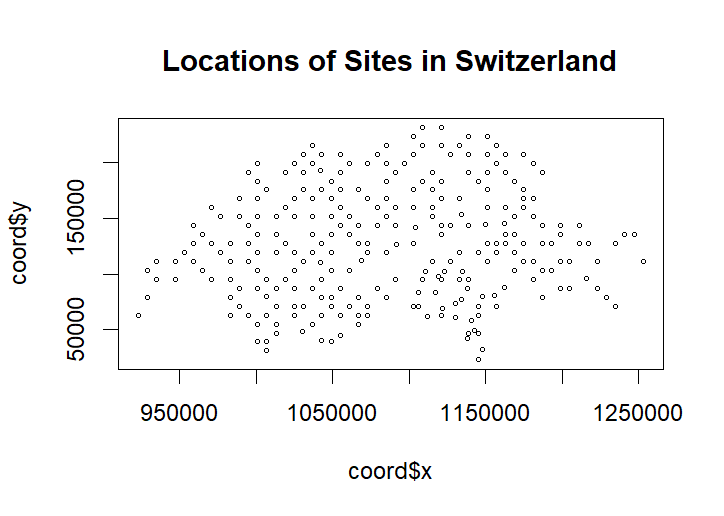
\includegraphics[width=3.5in,trim=.6cm 1.25cm .5cm .75cm, clip]{locations.png}  \caption{Locations of the 267 1km by 1km square quadrats laid out across the entirety of Switzerland in the MHB survey.  In general, the spacing of locations supports the use of an areal data model with neighbors defined through an adjacency matrix $A$.}
  \label{figure:locs}
\end{figure}

The response is the observed detection ($Y^{(s)}_{itv}=1$) or not ($Y^{(s)}_{itv}=0)$ of species $s$ at location $i$, time period $t$ and survey $v$. There were 266 to 267 sites observed in each season, with the number of surveys per season varying from 2 to 3.  Covariates on occupancy in $\bfX$ include the standardized percentage of forest cover at the location as well as the standardized elevation. The latent variable presence $Z^{(s)}_{it} = 1$ indicates that species $s$ was present at location $i$ and time period $t$, with detection probability $p^{(s)}_{it}$ modeled with standardized covariate duration, which measures the length of the particular survey.  Histograms of the values for the covariates are shown in Figure \ref{figure:covar}.  These same covariates are plotted across space in Figure \ref{figure:covar2}.  The left column shows raw data, and the right column shows interpolated covariates using a thin plate spline for ease of visualization only.

\begin{figure}[htbp]
  \centering
  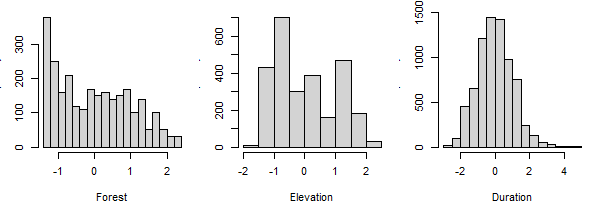
\includegraphics[width=5.5in]{hist.png}
  \caption{Histograms of the three covariates.  Left: Percent forest cover across the 267 locations. Center: Elevation of the 267 sites. Right:  Durations of the unique surveys.  Each coavariate is standardized and therefore unitless on this scale.}
  \label{figure:covar}
\end{figure}

\begin{figure}[ht]
  \centering
  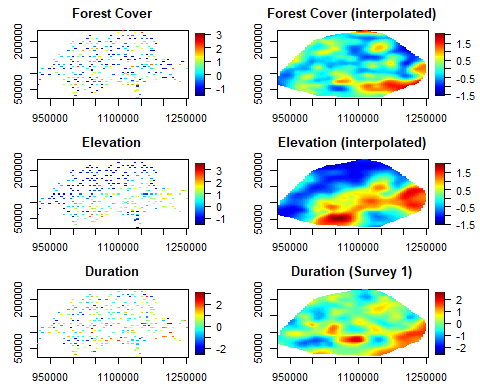
\includegraphics[width=5.5in]{eda.png}
  \caption{Spatial plots of the three covariates forest cover, elevation, and duration.  The left column shows raw data, and the right column shows interpolated data using a thin plate spline for ease of visualization only.  Forest and Duration are shown for season one, as these two covariates vary in time.}
  \label{figure:covar2}
\end{figure}

To define the neighborhood structure used for the spatial random effect, we selected a threshold of 15000 (meters, as these are UTM coordinates) and defined any two locations whose distance is less than 15000 to be neighbors. This threshold gave each location somewhere between 1 and 8 neighbors, with an average of 4.23 neighbors.  We assume $q=10$ spatial basis functions in each season.

The \code{multioccbuild(detection, occupancy, coords, DataNames, threshold)} function takes five arguments as input, and outputs \samp{model.input} which is then an argument for \code{GibbsSampler()} which implements the Gibbs Sampling MCMC algorithm to simulate from the posterior distribution.  Examples of the inputs \samp{occupancy}, \samp{detection},  \samp{coords}, \samp{DataNames} and \samp{threshold} for our application are shown below:

\begin{alltt}
> head(occupancy, n=4L)
  site season       forest        elev
1 Q001      1 -1.148171612 -1.14938671
2 Q002      1 -0.496936229 -1.14938671
3 Q003      1 -0.098959051 -0.21468405
4 Q004      1 -0.931093151 -0.37046783
\end{alltt}

\begin{alltt}
> head(detection, n=4L)
  site season survey Great.tit Blue.tit Coal.tit Crested.tit Marsh.tit Willow.tit   duration
1 Q001      1      1        NA       NA       NA          NA        NA         NA  0.1563255
2 Q002      1      1         1        1        0           0         1          0 -0.9274962
3 Q003      1      1         1        0        1           0         1          0 -0.2605290
4 Q004      1      1        NA       NA       NA          NA        NA         NA -0.8441253
\end{alltt}
Observe that some surveys have NAs for all detections.  Our model and package can easily accommodate missing values for the detections, but our model cannot handle missing values for occupancy covariates nor missing values for detection covariates when the corresponding `y` are not missing. Missing values in the covariates will result in a warning when the \code{multioccbuild()} function is run, and rows corresponding to those observations in \samp{detection} and possibly in \samp{occupancy} will be removed. We suggest that all quantitative variables to be used as detection or occupancy covariates be standardized to aid with mixing in the MCMC algorithm.  The remainder of the input items are:  

\begin{alltt}
> head(coords, n=4L)
  site      x      y
1 Q001 922942  63276
2 Q002 928942  79276
3 Q003 928942 103276
4 Q004 934942  95276
\end{alltt}

\begin{alltt}
> DataNames = list("species"=colnames(detection)[4:9],"detection"=c("duration"),
\hspace{1in} "occupancy"=c("forest","elev"))
> DataNames
\$species
[1] "Great.tit"   "Blue.tit"    "Coal.tit"    "Crested.tit" "Marsh.tit"   "Willow.tit" 

\$detection
[1] "duration"

\$occupancy
[1] "forest" "elev"
\end{alltt}
With each of these inputs properly defined, we run the main data function \code{multioccbuild()}:
\begin{alltt}
> model.input = multioccbuild(detection, occupancy, coords, DataNames, threshold = 15000)
Warning: Rows in detection with missing covariates have been removed for purposes of 
fitting the model, but the site/season combination is retained in occupancy and therefore 
predictions will be outputted.
\end{alltt}
The above message arises from cases in which we have NAs for covariates in detection $\bfW$, but we have actual observations of $y$ for these same site/season/survey combinations.  Our model cannot be fit using rows with missing detection covariates but non-missing detections in $y$.  There are 544 NAs in the covariate, but only 4 of these cases have non-missing detections: 
\begin{alltt}
> sum(is.na(detection\$duration))
[1] 544
> sum(!is.na(detection\$Great.tit) & is.na(detection\$duration))
[1] 4
\end{alltt}
One issue is site Q091, season 8:
\begin{alltt}
> detection[detection$site == "Q091" & detection$season==8,]
     site season survey Great.tit Blue.tit Coal.tit Crested.tit Marsh.tit Willow.tit  duration
5698 Q091      8      1         0        0        1           1         0          1 -1.177609
5965 Q091      8      2         1        0        1           1         0          1 -1.094238
6232 Q091      8      3         0        0        1           1         0          1        NA
\end{alltt}
The second issue is site Q125, season 2:
\begin{alltt}
> detection[detection$site=="Q125" & detection$season==2,]
     site season survey Great.tit Blue.tit Coal.tit Crested.tit Marsh.tit Willow.tit duration
926  Q125      2      1         1        1        1           1         1          0       NA
1193 Q125      2      2         1        1        1           0         1          0       NA
1460 Q125      2      3         1        1        1           1         1          0       NA
\end{alltt}
The \texttt{multioccbuild()} function replaces the observed occupancy data $y$ with NAs for these 4 cases.  The output is \samp{model.input}:
\begin{alltt}
model.input = list("DataNames"=DataNames,"X"=X,"W"=W,"y"=y,"A"=A,
"detection.info"=detection[,c("siteID","site","season","survey","observations")],
"occupancy.info"=occupancy[,c("siteID","site","season","x","y")])
\end{alltt}
Objects saved here reflect handling the missing data for the 4 rows described above:
\begin{alltt}
>model.input$y[(model.input$detection.info$site == "Q091" & 
model.input$detection.info$season == 8),]
     Great.tit Blue.tit Coal.tit Crested.tit Marsh.tit Willow.tit
5698         0        0        1           1         0          1
5965         1        0        1           1         0          1
6232        NA       NA       NA          NA        NA         NA

> model.input$y[(model.input$detection.info$site == "Q125" & 
model.input$detection.info$season == 2),]
     Great.tit Blue.tit Coal.tit Crested.tit Marsh.tit Willow.tit
926         NA       NA       NA          NA        NA         NA
1193        NA       NA       NA          NA        NA         NA
1460        NA       NA       NA          NA        NA         NA
\end{alltt}

The package reorders the data as site, then season, then survey, and ensures all matrices are in this order.  The resulting design matrices for occupancy $\bfX$ and detection $\bfW$ are

\begin{alltt}
> head(model.input\$X, n=4L)
          forest       elev
1  1 -1.14817161 -1.1493867
11 1 -0.49693623 -1.1493867
21 1 -0.09895905 -0.2146840
32 1 -0.93109315 -0.3704678

> nrow(model.input\$X)
[1] 2670

> head(model.input\$W, n=4L)
     [,1]       [,2]
[1,]    1  0.1563255
[2,]    1  1.1567763
[3,]    1  1.1567763
[4,]    1 -0.9274962

> nrow(model.input\$W) 
[1] 8010
\end{alltt}
The threshold is the Euclidean distance which defines whether or not two locations are neighbors.  In our, setting we set \texttt{threshold = 15000} which results in the $2670 \times 2670$ block diagonal adjacency matrix

\begin{alltt}
> model.input\$A[1:5,1:5]
   1 11 21 32 41
1  0  0  0  0  0
11 0  0  0  0  0
21 0  0  0  1  1
32 0  0  1  0  0
41 0  0  1  0  0
\end{alltt}

Observe the detections $\mathbf{y}$ are reordered because all components of the data were reordered according to site, season, and survey:

\begin{alltt}
> head(model.input\$y, n=4L)
    Great.tit Blue.tit Coal.tit Crested.tit Marsh.tit Willow.tit
1          NA       NA       NA          NA        NA         NA
268        NA       NA       NA          NA        NA         NA
535        NA       NA       NA          NA        NA         NA
2           1        1        0           0         1          0
\end{alltt}

\begin{alltt}
> head(model.input\$detection.info, n=4L)
    siteID site season survey observations
1        1 Q001      1      1            0
268      1 Q001      1      2            0
535      1 Q001      1      3            0
2        2 Q002      1      1            1
> nrow(model.input\$detection.info)
[1] 8010

> head(model.input\$occupancy.info, n=4L)
   siteID site season      x      y
1       1 Q001      1 922942  63276
11      2 Q002      1 928942  79276
21      3 Q003      1 928942 103276
32      4 Q004      1 934942  95276
> nrow(model.input\$occupancy.info)
[1] 2670
\end{alltt}

We ran our full analysis using the \code{GibbsSampler(M.iter = 50000, M.burn = 20000, \\M.thin = 10, model.input, q=10, sv=TRUE)}.  This took 4.03 hours to run on a single node on the Wake Forest University DEAC Cluster \citep{WakeHPC}.

Results from the analysis are shown in Tables \ref{tab:occ} and \ref{tab:det}.  It is important to note that we standardized all covariates to aid with MCMC mixing, and so we focus on the relative ordering of parameter estimates when comparing to other studies rather than absolute estimates.  Table \ref{tab:occ} shows the ordering of elevation's impact on occupancy as Willow Tit, Crested 
 and Coal Tit, Great Tit, Blue Tit and Marsh Tit.  This ordering largely matches the ordering published in \citet{tobler2019joint} (Table S2), which considered the same data and six species in a somewhat similar Joint Species Distribution Model.  \citet{chamberlain2016alpine} published that Willow Tits occupy higher elevations than Coal Tits in a nearby region of Italy, consistent with the ordering presented here.  Turning to percent forest cover, our results show higher occupancy with higher forest cover for the Willow, Coal and Crested Tits, middlling occupancy for Marsh Tit, and lower occupancy for the Great and Blue Tits, again matching the ordering of \citet{tobler2019joint}. 

\begin{table}[ht]
\centering
\begin{tabular}{rrrr}
  \hline
 Species & Intercept & Forest &  Elevation  \\ 
  \hline
Great Tit &  0.847 (0.769, 0.930) & -0.143 (-0.215, -0.072) & -0.224 (-0.300, -0.149) \\
Blue Tit  &  0.639 (0.547, 0.729) & -0.139 (-0.221, -0.058) & -0.261 (-0.349, -0.177) \\
Coal Tit  &  0.996 (0.919, 1.076) & -0.007 (-0.080,  0.066) & -0.130 (-0.204, -0.055) \\
Crested Tit & 0.764 (0.667 , 0.867) & -0.014 (-0.097,  0.071) & -0.138 (-0.223, -0.052) \\
Marsh Tit &  0.611 (0.509 , 0.724) & -0.124 (-0.219, -0.031) & -0.283 (-0.386, -0.182) \\
Willow Tit & 0.383 (0.267 , 0.506) &  0.108 (0.013,  0.199) &  0.068 (-0.028, 0.163) \\
   \hline
\end{tabular}
\caption{Posterior means and 95\% credible intervals for the occupancy regression coefficients $\bfalpha$.}
\label{tab:occ}
\end{table}

\begin{table}[ht]
\centering
\begin{tabular}{rrr}
  \hline
Species & Intercept & Duration  \\ 
  \hline
Great Tit  &  0.593 (0.553, 0.633) & -0.187 (-0.228, -0.147) \\
Blue Tit &     0.109 (0.069, 0.149) & -0.257 (-0.299, -0.214) \\
Coal Tit  &   0.738 (0.696, 0.779) &  0.303 (0.263, 0.346) \\
Crested Tit & -0.030 (-0.072, 0.011) &  0.352 (0.309, 0.395) \\
Marsh Tit &  -0.307 (-0.351, -0.264) & -0.090 (-0.133, -0.048) \\
Willow Tit & -0.482 (-0.532, -0.434) &  0.430 (0.377, 0.482) \\
   \hline
\end{tabular}
\caption{Posterior means and 95\% credible intervals for the detection regression coefficients $\bfbeta$}
\label{tab:det}
\end{table}

Turning next to the residual dependence structure, Figure \ref{figure:corr} shows the posterior mean of the correlation matrix computed from $\Sigma$ for the six species, with notable differences across pairs of species. We see a mixture of positive and negative correlations across different pairs of species, with, for instance, a strong positive signal for the Coal and Crested Tits but a strong negative correlation for the Willow and Marsh Tits. The positive correlation estimated here for Great tit and Blue tit is consistent with \citet{stenseth2015testing}, who noted these species occupy the same geographical areas and compete for resources, which can result in negative correlation for abundance, but positive correlation for occupancy. Our estimated correlations for the six species somewhat differ from those estimated by \citet{tobler2019joint}, who showed results on residual correlation of occupancy probability for the six tit species for a single season, but computed under a latent factor model. Their results showed all positive correlations among the six species, a result they noted with surprise.  However, this is reflective of the factor model structure in their assumed model which is less flexible than the multivariate random effect we used here. They also assumed different covariates and only modeled a single season, and as both model's dependence structures are residual to covariate effects, the estimates are not readily comparable.

\begin{figure}[htbp]
  \centering
  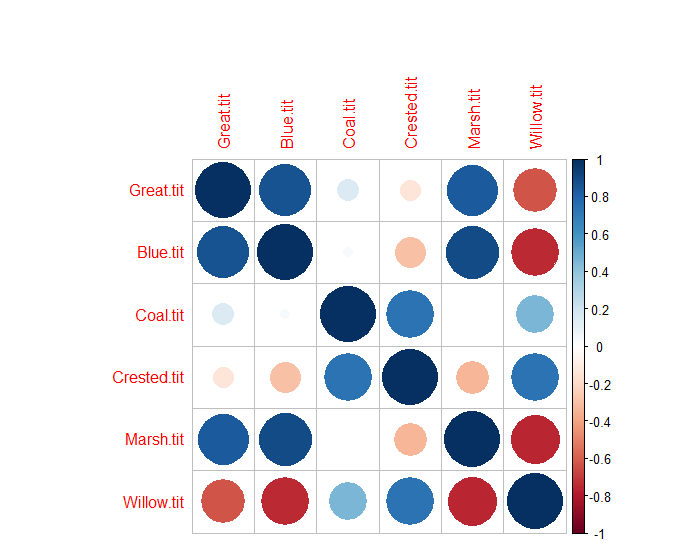
\includegraphics[trim= 0cm 0cm 0 1cm, clip, width=4.75in]{SigmaSharp.png}
  \caption{Posterior mean of the correlation matrix computed from $\Sigma$.  Plot shows examples of pairs of strongly correlated species (e.g. Great Tit and Blue Tit), strongly negative correlated species (e.g. Marsh Tit and Willow Tit), and largely uncorrelated species (e.g. Marsh Tit and Coal Tit).}
  \label{figure:corr}
\end{figure}

Figures \ref{figure:psi1} and \ref{figure:psi7} show posterior means for occupancy probabilities $\psi$ for seasons 1 and 7 for all six species. Hollow circles show the actual detections of each species in each corresponding season.  For all $T=10$ years, we observe a very strong relationship between predicted occupancy probabilities $\psi$ and species detections for all species and all seasons. 

\begin{figure}[ht]
  \centering
  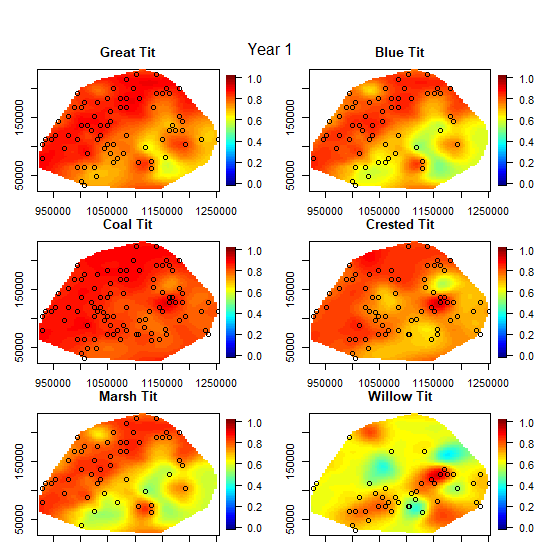
\includegraphics[width=5.5in]{psi1.png}
  \caption{An example of occupancy predictions for season 1.  Colors show posterior means of $\psi$ for each location and species, interpolated across space using a thin plate spline for ease of visualization only.  Hollow circles show points with detections of the species in that particular season.  As expected, regions of higher posterior probability match regions with greater density of detections.}
  \label{figure:psi1}
\end{figure}

\begin{figure}[ht]
  \centering
  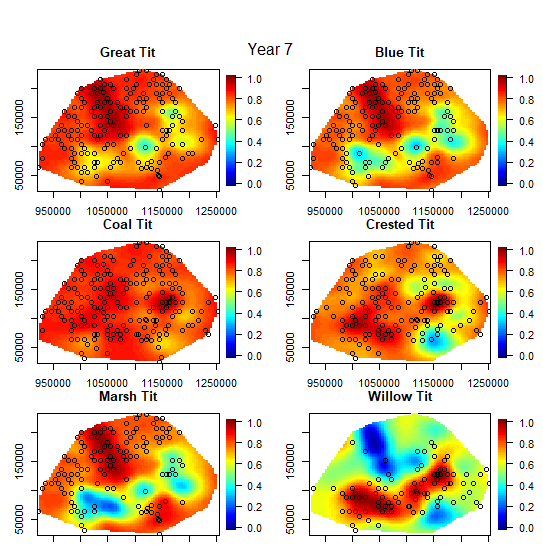
\includegraphics[width=5.5in]{psi7.png}
  \caption{An example of occupancy predictions for season 7.  Colors show posterior means of $\psi$ for each location and species, interpolated across space using a thin plate spline for ease of visualization only.  Hollow circles show points with detections of the species in that particular season.  As expected, regions of higher posterior probability match regions with greater density of detections.}
  \label{figure:psi7}
\end{figure}

\section{Conclusion}

In this article, we introduced the \texttt{R} package \pkg{multiocc} for implementing the multivariate spatio-temporal occupancy model proposed by \citet{hepler2021spatiotemporal}. This model overcomes many of the limitations of occupancy models that can be implemented with already existing \texttt{R} packages. More specifically, this model can jointly analyze $S \geq 1$ species over multiple seasons with a varying number of surveys at each site per season. The use of spatial basis functions makes this method feasible even with a large number of spatial locations. 

Using this package to analyze imperfectly detected presence/absence data requires two main steps. First, the \code{multioccbuild()} function takes the raw data and outputs all matrices required to run the MCMC algorithm. Then, the \code{GibbsSampler()} function performs the Gibbs sampling algorithm to generate samples from the posterior distribution which can then be used to perform inference. We illustrated use of this package by analyzing occupancy data on six bird species in Switzerland from 2004 - 2013. The development of \pkg{multiocc} makes this multivariate spatio-temporal occupancy model accessible to the large community of researchers who use \texttt{R} for their data analysis needs. 



\hypertarget{refs}{}

\bibliography{RJreferences.bib}

\address{%
Staci Hepler\\
Department of Statistical Sciences, Wake Forest University\\%
Winston-Salem NC, 27103 USA\\
%
%
%
\href{mailto:heplersa@wfu.edu}{\nolinkurl{heplersa@wfu.edu}}%
}

\address{%
Robert Erhardt\\
Department of Statistical Sciences, Wake Forest University\\%
Winston-Salem NC, 27103 USA\\
%
%
%
\href{mailto:erhardrj@wfu.edu}{\nolinkurl{erhardrj@wfu.edu}}%
}
